% !TeX root = ./presentazione.tex
% !TeX encoding = UTF-8 Unicode
% !TeX spellcheck = it_IT
% !TeX program = arara
% !TeX options = --log --verbose --language=it "%DOC%"

% arara: lualatex: { interaction: batchmode }
% arara: lualatex: { interaction: nonstopmode, synctex: yes }

\documentclass[
  usepdftitle=false,
  % notes,
  bigger,
  aspectratio=169,
  lualatex,
  % handout,
  italian
]{beamer}

\usepackage{pgfpages}
\usepackage{fontspec}
\defaultfontfeatures{Ligatures={TeX}}
\usepackage[
  output-decimal-marker={,},
  binary-units
]{siunitx}
\usepackage[%
  strict=true,
  autostyle=true,
  english=american,
  italian=guillemets
]{csquotes}
\usepackage{polyglossia}
\setmainlanguage[babelshorthands]{italian}
\setotherlanguage[variant=american]{english}
\usepackage{graphicx}
% \usepackage{svg}
% \usepackage{tikz}
% \usepackage{multimedia}
\usepackage{media9}
% \usepackage{minted}
\usepackage[
  subrefformat=parens,
  labelformat=parens
]{subcaption}
\usepackage{caption}
\usepackage{adjustbox}
\usepackage{microtype}

\hypersetup{%
  pdftitle={Progettazione di una piattaforma web per la simulazione di programmi aggregati},
  pdfauthor={Niccolò Maltoni},
  pdfsubject={La programmazione aggregata è un approccio innovativo nato in tempi recenti per far fronte alla necessità di un punto di vista nuovo nella programmazione di sistemi distribuiti. In particolare, basandosi sull'impianto teorico del field calculus, negli ultimi anni sono stati realizzati, da parte dell'Università di Bologna, linguaggi e framework innovativi per la sua applicazione in contesti d'uso reale: Protelis e ScaFi. La principale criticità che mina la diffusione di questo tipo di linguaggi è legata alla configurazione del sistema per l'esecuzione: è infatti necessario avere a disposizione una rete, reale o fisica, di dispositivi per l'esecuzione del codice e, soprattutto in contesto didattico, la necessità di dispiegare un certo numero di dispositivi o configurare un simulatore può costituire un ulteriore gradino di complessità. Lo scopo di questa tesi è progettare una piattaforma web che permetta di realizzare semplici programmi aggregati senza configurazione alcuna. È stato realizzato un sistema composto da un server esecutore, che si avvale del simulatore Alchemist per eseguire il codice Protelis, e da un'applicazione web in React che permetta la scrittura del codice e il monitoring dell'esecuzione.},
  pdfkeywords={Aggregate computing, Aggregate programming, Protelis, Applicazione web, Simulazione},
  pdfpagemode={UseNone},
  hidelinks,
  hypertexnames=false,
  linktoc=all,
  unicode=true,
  pdftoolbar=false,
  pdfmenubar=false,
  plainpages=false,
  breaklinks,
  pdfstartview={Fit},
  pdflang={it}
}

\usetheme{Boadilla}
\usecolortheme{beaver}
\setbeameroption{hide notes} % Only slide
%\setbeameroption{show only notes} % Only notes
%\setbeameroption{show notes on second screen=right} % Both
\setbeamertemplate{note page}[plain]
\beamertemplatenavigationsymbolsempty
\hypersetup{pdfpagemode=UseNone} % don't show bookmarks on initial view
% \setbeamertemplate{items}[triangle]

\title[WebProtelis]{%
  Progettazione di una piattaforma web per la\\simulazione di programmi aggregati%
}

\subtitle{Tesi in Pervasive Computing}

\author[Niccolò~Maltoni (0000840825)]{%
  Niccolò~Maltoni%
  \\\small{Matricola: 0000840825}%
  \\\vspace{10pt} \small{Realtore: Prof.~Mirko~Viroli \\Correlatore: Prof.~Danilo~Pianini}
}

\institute[]{%
  Alma Mater Studiorum - Università di Bologna\\%
  Campus di Cesena%
}

\date{19 marzo 2020}

% %% Permette di inserire l'outline prima di ogni sezione
% \AtBeginSection[]{%
%   \begin{frame}<beamer>
%     \frametitle{Outline}
%     \tableofcontents[currentsection]
%   \end{frame}
% }

\begin{document}

  \frame{\titlepage}

  % \begin{frame}<beamer>
  %   \frametitle{Outline}
  %   \tableofcontents
  % \end{frame}

  \section{Introduzione}
  \subsection{Obiettivo}
  \begin{frame}{\insertsection}{\insertsubsection}

    Lo scopo di questa tesi è progettare una piattaforma web che permetta di realizzare semplici programmi aggregati senza configurazione alcuna.

    \medskip
    \pause

    È stato realizzato un sistema composto da un server esecutore, che si avvale del simulatore Alchemist per eseguire il codice Protelis,
    e da un'applicazione web in React che permetta la scrittura del codice e il \emph{monitoring} dell'esecuzione.

  \end{frame}

  \section{Background}
    \subsection{Stato dell'arte}

      \begin{frame}{\insertsectionhead}{\insertsubsectionhead}
        \begin{columns}
          \begin{column}{.7\textwidth}
            \begin{block}<1->{Programmazione aggregata}
              La programmazione aggregata costituisce un'alternativa all'approccio ``classico'' volta a semplificare la progettazione, creazione e manutenzione di sistemi distribuiti complessi.
            \end{block}

            \begin{columns}
              \begin{column}{.8\textwidth}
                \begin{block}<2->{Linguaggi}
                  \begin{itemize}
                    \item<2-> \strong{Protelis}
                    \item<3-> ScaFi
                  \end{itemize}
                  \onslide<4->{Entrambi eseguono su JVM}
                \end{block}
              \end{column}
              \begin{column}{.15\textwidth}
                \begin{figure}
                  \includegraphics<2->[width=\textwidth]{../res/fig/protelis-logo.png}
                \end{figure}
              \end{column}
            \end{columns}
          \end{column}
          \begin{column}{.25\textwidth}
            \begin{figure}
              \includegraphics<1->[height=.7\textheight]{res/fig/stack-partial.eps}
            \end{figure}
          \end{column}
        \end{columns}
      \end{frame}

      % \begin{frame}{\insertsectionhead}{\insertsubsectionhead}
      %   \begin{columns}
      %     \begin{column}{.8\textwidth}
      %       \begin{block}{Protelis}
      %         \begin{itemize}[<+->]
      %         \item
      %             Linguaggio di programmazione basato sul paradigma aggregato fortemente influenzato da \emph{Proto}
      %           \item
      %             Incorpora le principali funzionalità di computazione spaziale della programmazione aggregata
      %           \item
      %             Possiede una sintassi più simile ai linguaggi strutturati tradizionali come C o Java
      %           \item
      %             È \emph{Java-hosted}
      %             \begin{itemize}
      %               \item richiede un ambiente JVM in cui eseguire l'interprete
      %             \end{itemize}
      %         \end{itemize}
      %       \end{block}
      %     \end{column}
      %     \begin{column}{.15\textwidth}
      %       \begin{figure}
      %         \includegraphics[width=\textwidth]{../res/fig/protelis-logo.png}
      %       \end{figure}
      %     \end{column}
      %   \end{columns}
      % \end{frame}

    \subsection{Problematica}

    \begin{frame}{\insertsectionhead}{\insertsubsectionhead}
      \begin{columns}
        \begin{column}{.6\textwidth}
          \begin{alertblock}{\insertsubsectionhead}
            \begin{itemize}
              \item<1->
                Il linguaggio richiede una rete di dispositivi su cui eseguire:
                \begin{itemize}
                  \item<2-> rete fisica
                  \item<3-> NASA WorldWind
                  \item<4-> ProtelisVM
                  \item<5-> Alchemist
                \end{itemize}
            \end{itemize}
          \end{alertblock}
        \end{column}
        \begin{column}{.35\textwidth}
          \begin{figure}
            \centering
            \includegraphics<2>[width=.85\textwidth]{res/fig/network.png}
            \includegraphics<3 | handout 0>[width=.85\textwidth]{res/fig/nasaworldwind.png}
            \includegraphics<4 | handout 0>[width=.85\textwidth]{res/uml/protelis-vm.eps}
            \includegraphics<5 | handout 0>[width=.85\textwidth]{res/fig/alchemist.png}
            \includegraphics<6 | handout 0>[width=.85\textwidth]{res/fig/protelis-alchemist-arch.eps}
          \end{figure}
        \end{column}
      \end{columns}
    \end{frame}

    \subsection{Requisiti e casi d'uso}

    \begin{frame}{\insertsectionhead}{\insertsubsectionhead}
      \begin{columns}
        \begin{column}{.5\textwidth}
          \begin{block}{Requisiti}
            \begin{itemize}
              \item
                Progettare un sistema che permetta di iniziare a utilizzare Protelis senza configurazioni
                \begin{itemize}
                  \item nessun build-script
                  \item nessun deploy di dispositivi
                \end{itemize}
              \item
                L'utente si assume essere inesperto della piattaforma
                \begin{itemize}
                  \item l'interfaccia deve essere semplice e immediata
                \end{itemize}
              \item La piattaforma dovrebbe essere accessibile tramite browser
            \end{itemize}
          \end{block}
        \end{column}
        \begin{column}{.45\textwidth}
          \begin{figure}
            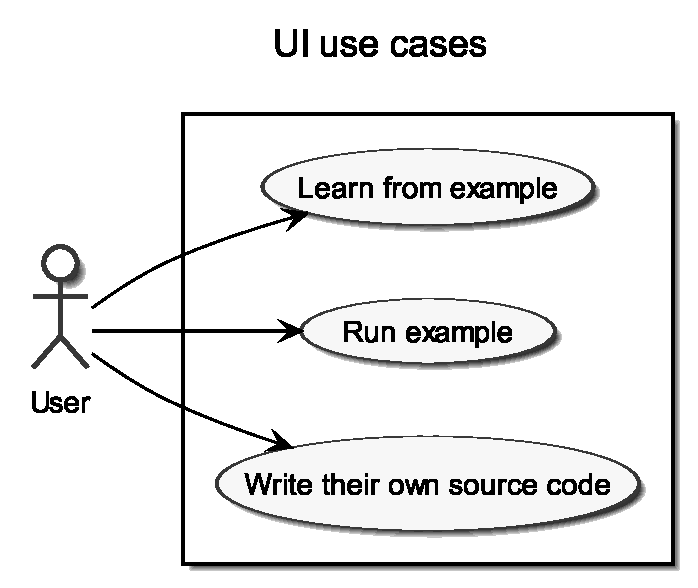
\includegraphics[width=\textwidth]{res/uml/use-cases-frontend.eps}
          \end{figure}
        \end{column}
      \end{columns}
    \end{frame}

    \begin{frame}{\insertsectionhead}{\insertsubsectionhead}

      \begin{block}{Analisi del problema}
        \begin{itemize}
          \item
            non è possibile eseguire un interprete Protelis all'interno della sandbox un browser
            \begin{itemize}
              \item le Java applet sono deprecate da tempo
            \end{itemize}
          \item
            è necessario suddividere l'architettura in due componenti
            \begin{itemize}
              \item un'interfaccia Single-Page accessibile tramite browser
              \item un server esecutore accessibile tramite API dal client
            \end{itemize}
        \end{itemize}
      \end{block}

      \begin{figure}
        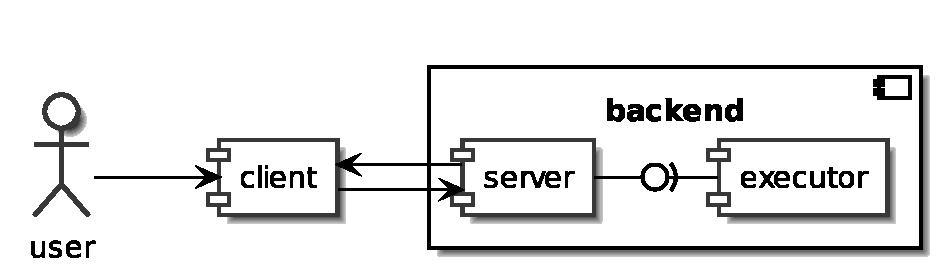
\includegraphics[width=.71\textwidth]{../res/uml/architecture-design.eps}
      \end{figure}

      % \begin{figure}
      %   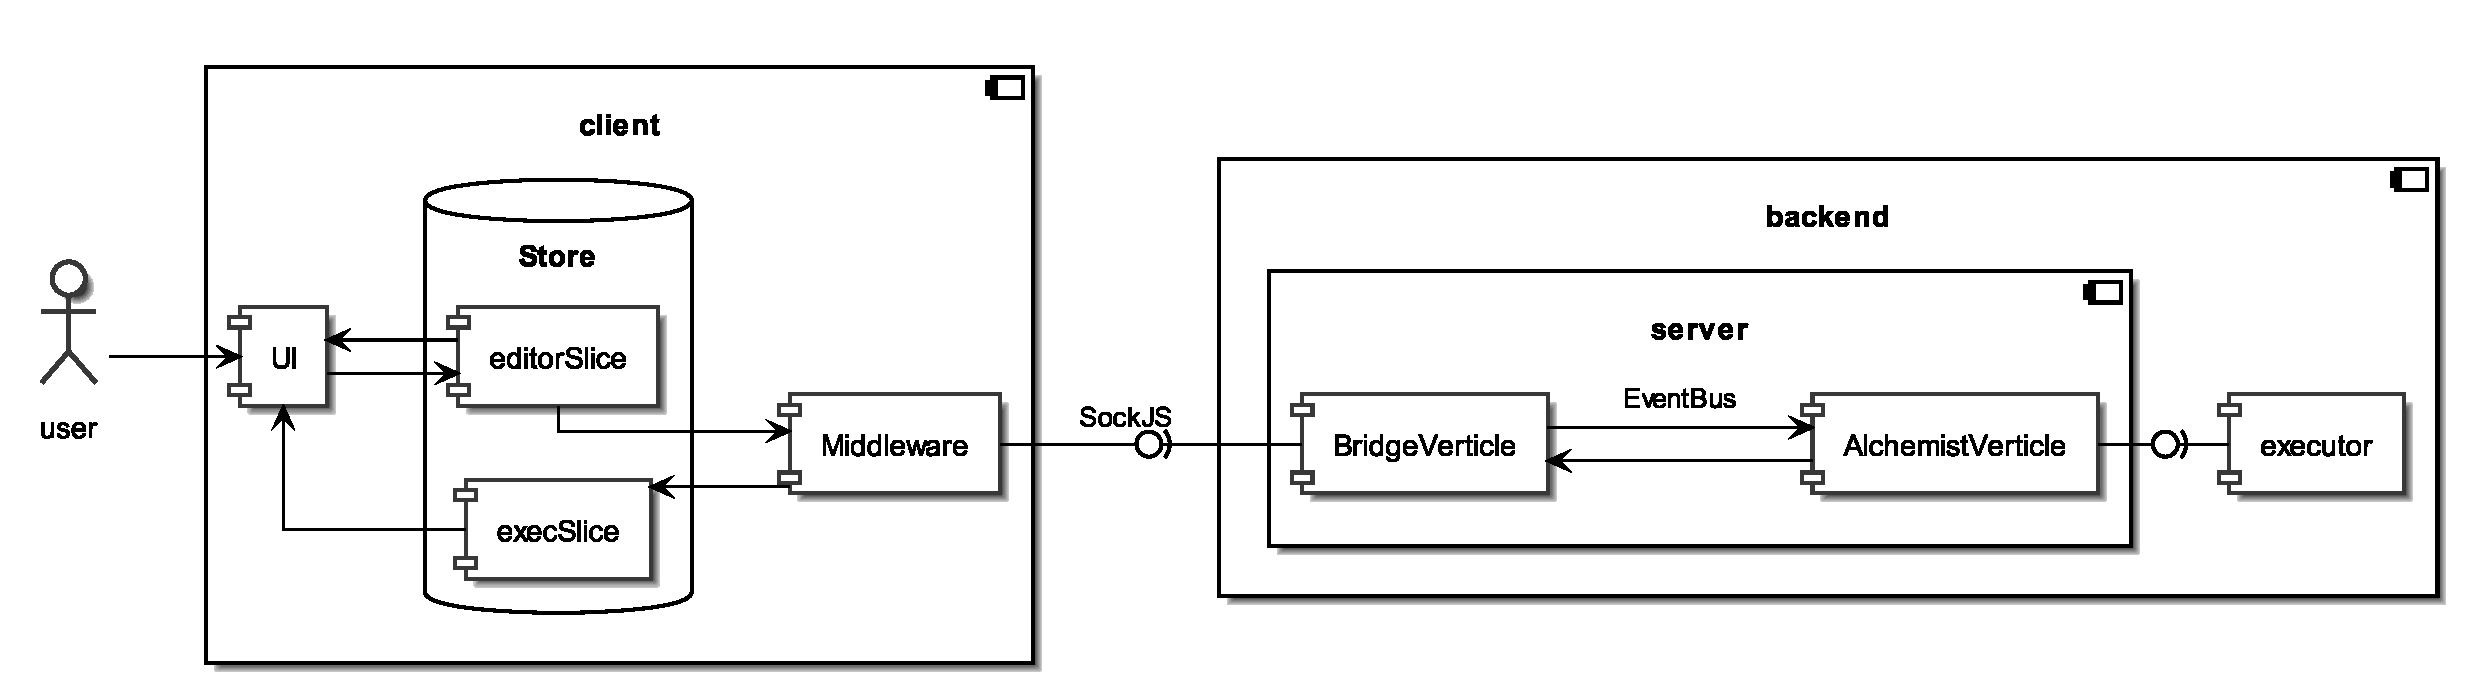
\includegraphics[width=.69\textwidth]{res/uml/architecture-design-detail.eps}
      % \end{figure}
    \end{frame}

  \section{WebProtelis}

  \begin{frame}{\insertsectionhead}
    \begin{figure}
      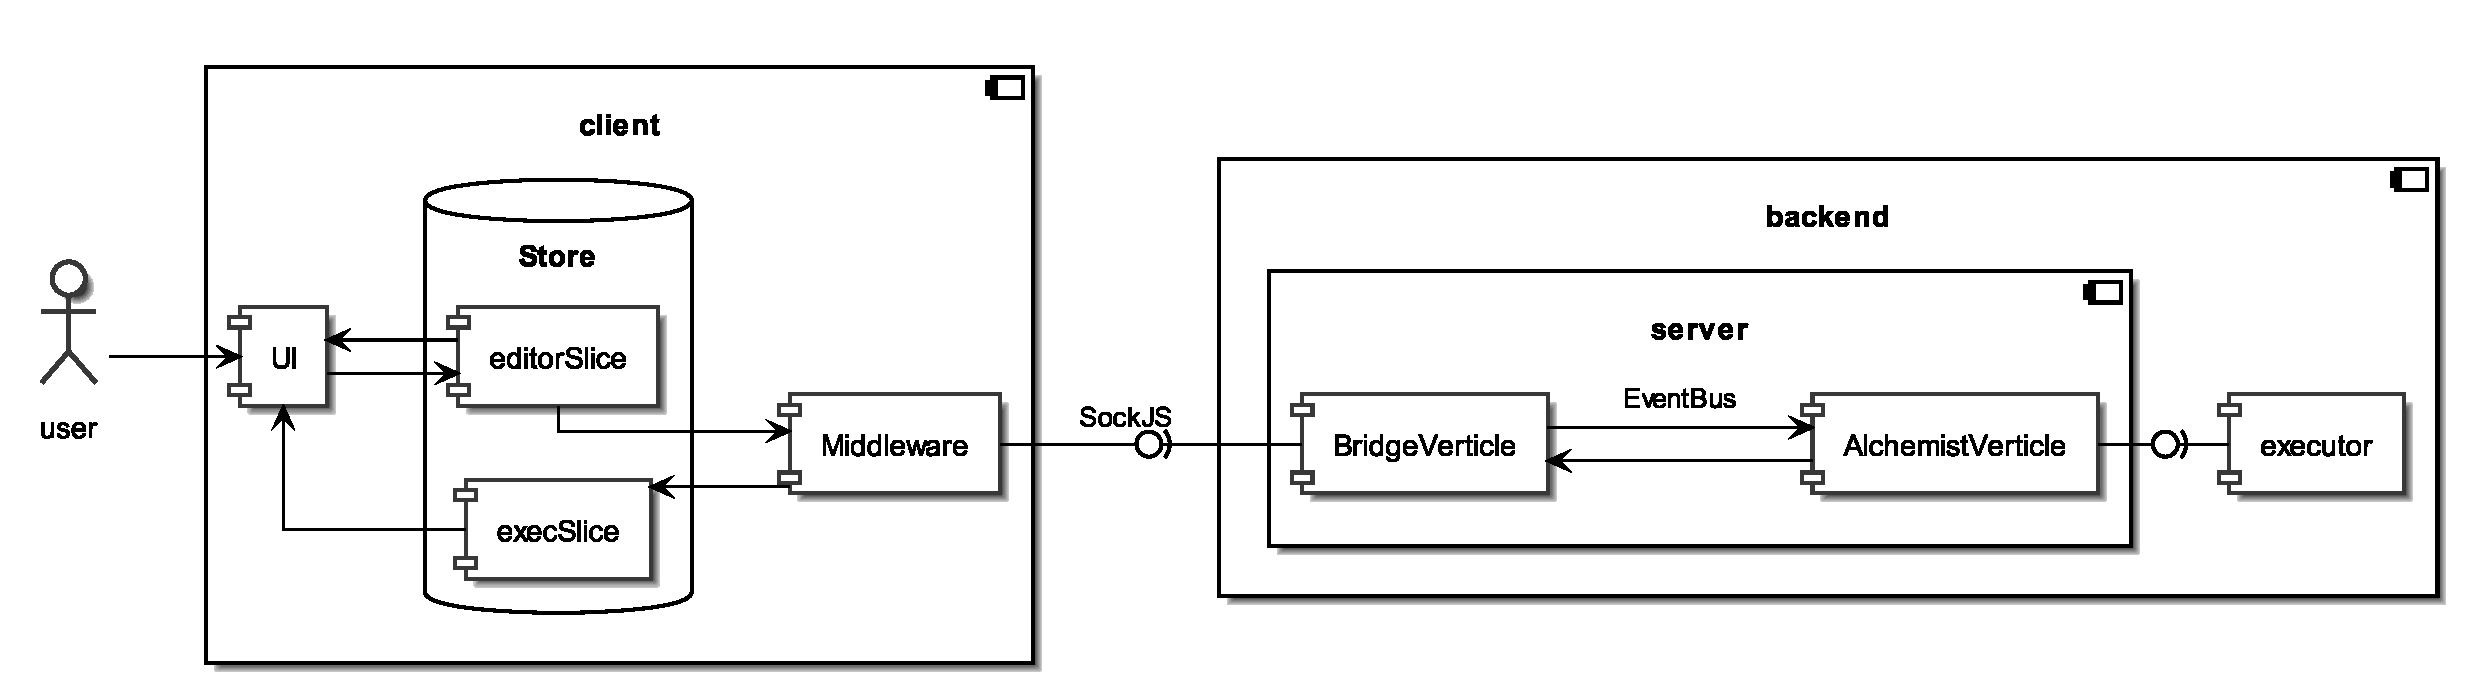
\includegraphics[width=\textwidth]{res/uml/architecture-design-detail.eps}
    \end{figure}
  \end{frame}

  \subsection{Progettazione del server}

    \begin{frame}{\insertsectionhead}{\insertsubsectionhead}

      \begin{block}{Servizi offerti}
        Il backend è composto da due entità principali
        \begin{itemize}
          \item server che espone API per la comunicazione remota
          \item esecutore del codice Protelis
        \end{itemize}
      \end{block}

      \begin{block}{Scelte tecnologiche}
        \begin{itemize}
          \item Vert.x      % TODO: spiega meglio
          \item Kotlin      % TODO: spiega meglio
          \item Alchemist   % TODO: spiega meglio
        \end{itemize}
      \end{block}
    \end{frame}

    \begin{frame}{\insertsectionhead}
      \framesubtitle{\insertsubsectionhead}

      \begin{block}{Vert.x}
        \strong{Vert.x} è un framework applicativo reattivo e event-driven per JVM.

        Caratteristiche principali:
        \begin{itemize}
          \item<1-> reattivo e basato su pattern Multi-Reactor
          \item<2-> supporto a costrutti \emph{actor-like} detti \strong{Verticle}
          \item<3-> supporto a comunicazione tramite EventBus
        \end{itemize}

        % Del modello architetturale messo a disposizione dal framework, è stato considerato interessante il concetto di \emph{Verticle}:
        % esso è un'astrazione, simile al pattern ad attori ma non considerato pienamente aderente al modello teorico dalla stessa documentazione ufficiale,
        % che incapsula un event-loop insieme al suo stato e interagisce tramite gli eventi provenienti da un EventBus.
      \end{block}

      % \begin{block}<1>{Pattern reactor}
      %   Pattern di gestione degli eventi tramite event-loop, il quale utilizza degli handler per gestire gli eventi in una coda
      % \end{block}

      \begin{block}<4->{Verticle modellati}
        \begin{itemize}
          \item \texttt{BridgeVerticle} gestisce le API attraverso \emph{SockJS} e \emph{EventBus}
          \item \texttt{AlchemistVerticle} costruisce e monitora simulazioni Alchemist per eseguire il codice Protelis
        \end{itemize}
      \end{block}
    \end{frame}

    \begin{frame}{\insertsectionhead}
      \framesubtitle{\insertsubsectionhead}

      \begin{block}{Alchemist}
        \begin{itemize}
          \item<1-> Alchemist è un meta-simulatore \textbf<2->{estendibile} \emph{open-source} che esegue su JVM, nato all'interno dell'Università di Bologna.
          \item<2-> Offre un'\emph{incarnazione} che permette di simulare reti di dispositivi che possono eseguire codice Protelis
        \end{itemize}
      \end{block}
    \end{frame}

    \subsection{Progettazione del client}

    \begin{frame}{\insertsectionhead}{\insertsubsectionhead}
      \begin{block}{Struttura}
        \begin{itemize}
          \item<1-> Il client dovrebbe essere una Single-Page Application composta da un editor e da un canvas
          \item<2-> Simile a CodeSandbox\onslide<3->{, TypeScript Playground }\onslide<4->{o Overleaf}
        \end{itemize}
      \end{block}

      \begin{figure}
        \centering
        \only<2>{%
          \includegraphics[width=.5\textwidth]{res/fig/codesandbox.png}%
        }%
        \only<3>{%
          \includegraphics[width=.5\textwidth]{res/fig/typescript-playground.png}%
        }%
        \only<4>{%
          \includegraphics[width=.5\textwidth]{../res/fig/overleaf.png}%
        }%
      \end{figure}
    \end{frame}

    \begin{frame}{\insertsectionhead}{\insertsubsectionhead{}: Mockup}
      \centering
      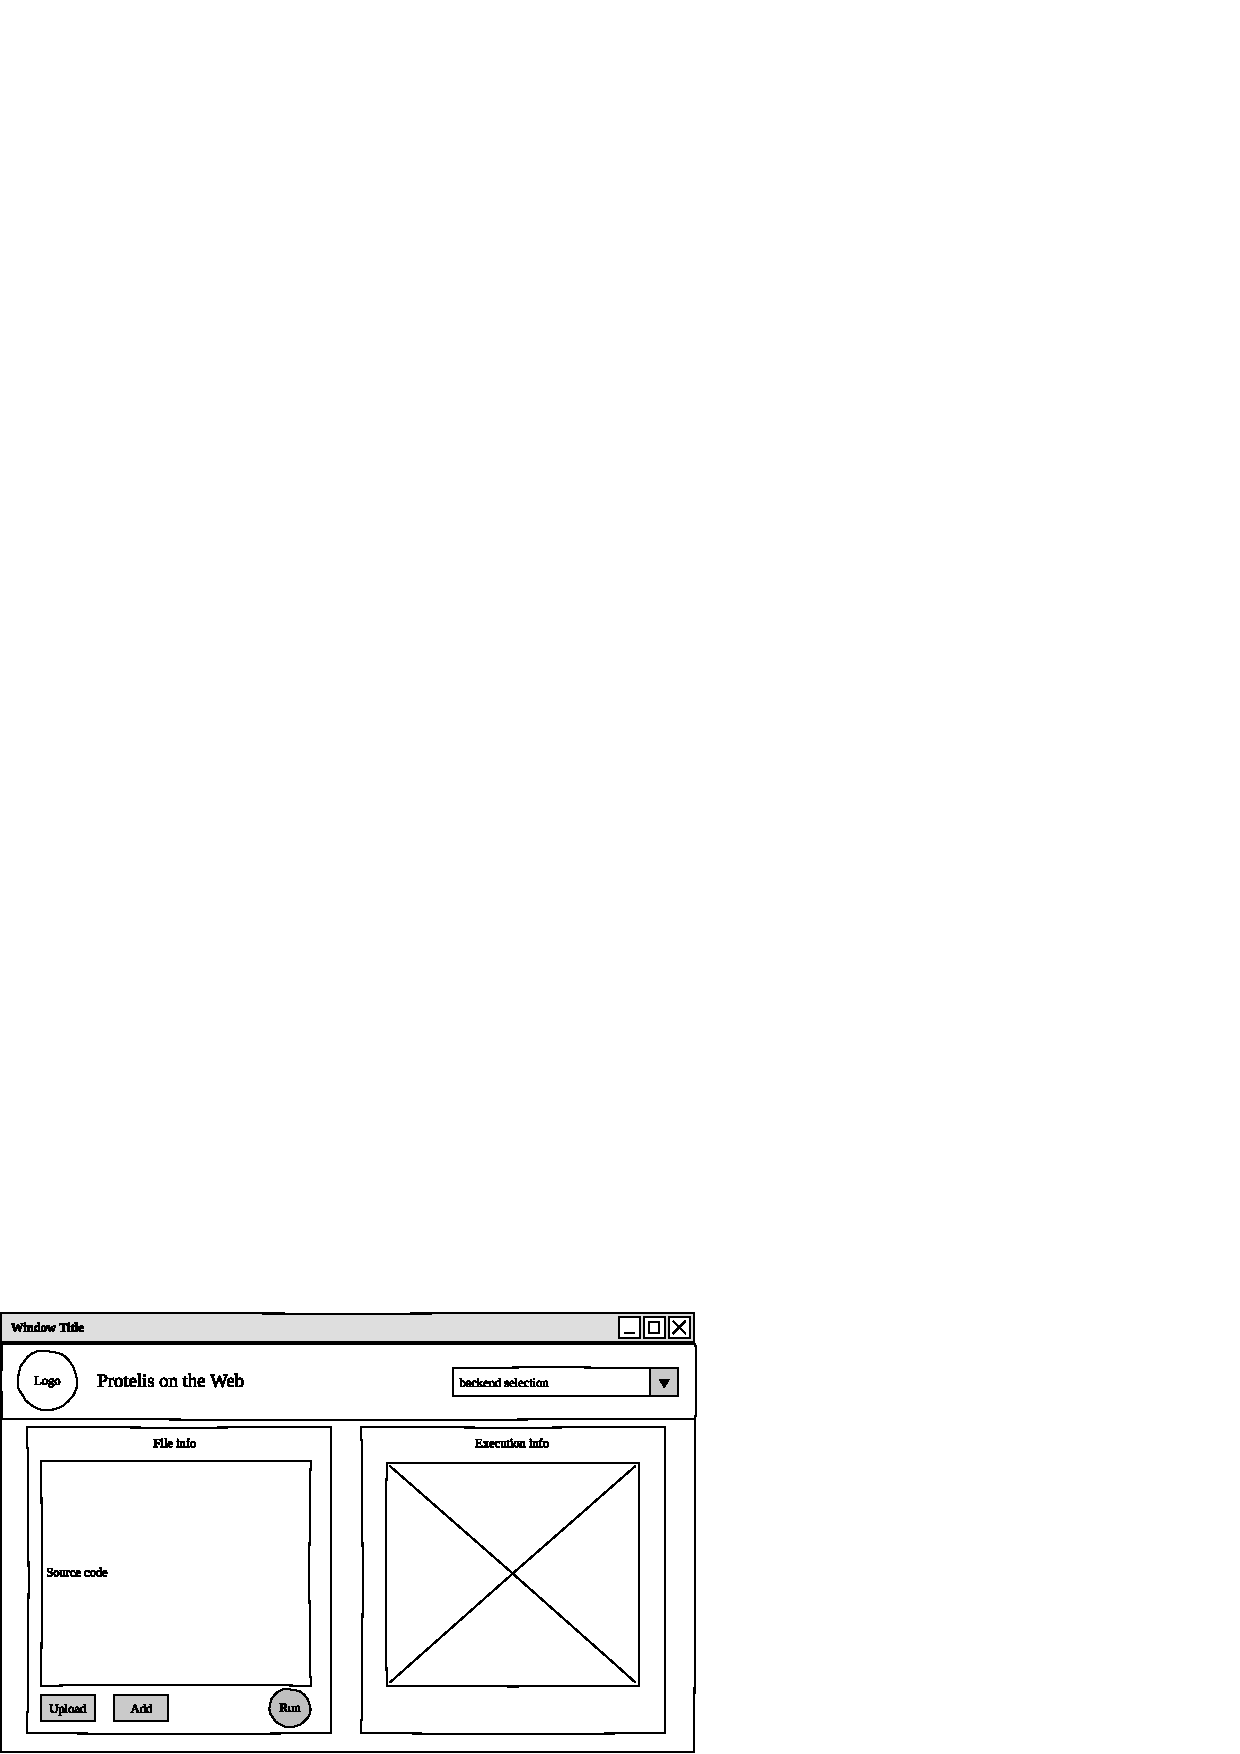
\includegraphics[width=.9\textwidth]{res/fig/gui-actual.png}
    \end{frame}

    \begin{frame}{\insertsectionhead}{\insertsubsectionhead}
      \begin{block}{Framework}
        \begin{itemize}
          \item
            Per l'implementazione è stato scelto \strong{React}
            \begin{itemize}
              \item React è una libreria per la costruzione di pagine web reattive e data-driven
              \item Suddivide la pagina in componenti, gestiti tramite struttura ad albero
              \item Tramite un sistema di dipendenze, determina in modo reattivo cosa deve essere renderizzato nuovamente
            \end{itemize}
          \item Fondamentale pianificare la gestione dello \strong{stato}
          % \item
          %   Come linguaggio di programmazione è stato scelto TypeScript
          % \item
          %   Per la gestione dello stato si è deciso di utilizzare Redux
        \end{itemize}
      \end{block}

      % TODO: inserisci immagini
    \end{frame}

    \begin{frame}{\insertsectionhead}{\insertsubsectionhead}
      \begin{block}{Gestione dello stato}
        \begin{itemize}
          \item<1-> Come alternativa a MVC Facebook propone per le applicazioni React un nuovo pattern architetturale: \strong{Flux}
          \item<2-> \strong{Redux} è una delle più popolari varianti del pattern Flux
        \end{itemize}
      \end{block}

      \begin{figure}
        \centering
        \only<1>{%
          \includegraphics[width=.65\textwidth]{../res/fig/flux-diagram-white-background.png}%
        }%
        \only<2>{%
          \includegraphics[width=.65\textwidth]{../res/fig/redux-diagram.png}%
        }%
      \end{figure}
    \end{frame}

    \begin{frame}
      \begin{block}{Componenti e stato}
        Sono state individuate due \emph{slice} dello stato, relativamente ai due elementi di layout principali:
        \begin{itemize}
          \item<2-> \texttt{editorSlice}
          \item<3-> \texttt{execSlice}
        \end{itemize}
      \end{block}

      \begin{figure}
        \centering
        \only<2>{%
          \includegraphics[width=.65\textwidth]{../res/screenshot/Screenshot_2020-03-02 Protelis on the Web(2).png}%
        }%
        \only<3>{%
          \includegraphics[width=.65\textwidth]{../res/screenshot/Screenshot_2020-03-02 Protelis on the Web(7).png}%
        }%
      \end{figure}
    \end{frame}

  \subsection{Valutazione dei risultati}

    \begin{frame}{\insertsectionhead}{\insertsubsectionhead{}: Demo}
      \centering
      \includemedia[%
        width=.9\textwidth,%
        height=.5\textwidth,%
        keepaspectratio,%
        activate=pageopen,%
        passcontext,%
        transparent,%
        addresource=res/demo.mp4,%
        flashvars={source=res/demo.mp4}%
      ]{}{VPlayer.swf}
    \end{frame}

    \begin{frame}{\insertsectionhead}{\insertsubsectionhead{}: LightHouse}
      \centering
      \includegraphics[width=.9\textwidth]{../res/tests/Screenshot_2020-03-04 Lighthouse Report Viewer.png}
    \end{frame}


  \section{Conclusioni}

  \begin{frame}{\insertsectionhead}
    L'obiettivo della tesi è stato per la maggior parte raggiunto:
    il prototipo realizzato rispetta i requisiti e l'architettura progettata lascia aperte numerose possibilità di espansione.

    % \pause
    \bigskip

    Il sistema sviluppato si basa su Alchemist per la simulazione della rete di dispositivi, ma supporta diversi possibili backend.
    Un esempio notevole è l'impiego di una rete di dispositivi fisici o una rete ibrida:
    in questo particolare caso, il sistema potrebbe permettere un monitoring del sistema dispiegato nell'ambiente reale.
  \end{frame}


  % \frame{\titlepage}

\end{document}
